\documentclass[12pt,german,a4paper]{scrartcl}
\linespread{1.2}
\usepackage{graphicx,url}
\usepackage{tikz,fancyhdr} 
\usepackage[sort&compress]{natbib}
\usepackage{color}

%\include{draft}
%\usepackage[ngerman]{babel}
\usepackage[utf8]{inputenc}
\usepackage[pdftex,plainpages=false,pdfpagelabels]{hyperref}

\usepackage{listings} %quelltext-listings
\lstset{basicstyle=\ttfamily\scriptsize}

\definecolor{blue}{rgb}{0.2,0.3,0.5}
\addtokomafont{section}{\color{blue}}
\addtokomafont{subsection}{\color{blue}}
\addtokomafont{subsubsection}{\color{blue}}

\hypersetup{
    pdftitle={Memory Tool Documentation},
    pdfauthor={Hagen Fritsch and Dominik Meyer}
}

\title{Memory Tool Documentation}
	
\newcommand{\q}[1]{\glqq{#1}\grqq}
%\newcommand{\citet}{\emcite}

\begin{document}
%titelseite und inhalt
\pagenumbering{roman}
\thispagestyle{empty}
\begin{center}
	\sffamily {\huge \textbf{\color{blue} Memory Tool Documentation}}
	\begin{flushleft}
		Hagen Fritsch \texttt{\small <fritsch+mdp@in.tum.de>} \hfill
		Technische Universität München \\
		Dominik Meyer  \texttt{\small <meyerd@in.tum.de>} \hfill August 1st, 2009
	\end{flushleft}
\end{center}

%\setcounter{page}{2}
%\thispagestyle{empty}
\tableofcontents{}
%\listoftables

%\newpage
\pagenumbering{arabic}

%%%%%%%%%%%%%%%%%%%%
\vfill
\section*{Abstract}
The goal of the project is to compare two memory images of one virtual machine and extract a high-level view
of changes in kernel data structures, which is achieved through structured and typed memory based inspection
on debug-symbols of the Linux kernel.
The results of the comparison shall be the base for a machine-learning approach to identify
malicious behaviour based solely on passive memory observation.

	\section{Overview}
In a first step of meaningful virtual machine memory introspection, the exact semantics of all data in memory need to be known,
which seems like an impossible task at the first glance, but fortunately access to memory semantics is essential for
other tasks (mainly debugging) and thus a lot of required information can be obtained with ease.
When compiling a binary, the compiler can be told to add debug information, describing data types and structures,
which is fundamental for accessing memory in meaningful ways. Additionally, the debug information will note the addresses
of global variables. These are going to be the entry points for memory inspection, as they allow us to recursively
follow typed information such as structures and pointers through memory.
Though there are still many obstacles to overcome, this approach is a giant first step in full memory inspection.

In order to access not only flat kernel memory, but complete paged memory, paging is being implemented in a second stage of the project, before eventually measures to analyse changes between two memory dumps can be initiated.

By using the outcome of this analysis we were able to inspect if the effects of installing rootkits into the kernel can be observed. Our conclusions can be found in chapter \ref{rootkit_analysis}.

\newpage

	\section{Data acquirement process}
Debug kernel images contain all information needed for memory inspection in a binary format. However, as implementing a parser to access the binary format debug symbols seemed unreasonable due to elf’s complexity and likelihood of being subject to change, the decision was made to not work on the raw data, but to parse \texttt{objdump}’s output of the debug symbols which has some advantages.

\begin{description}
	\item[Size reduction] A debug kernel image is usually around 50 to 100 mb in size, while the parsed and cleaned debug symbols are only around 15 mb.
	\item[Redundancy reduction] The main reason for size reduction is, that most redundancies in the symbols have been removed. The kernel image tends to contain many duplicate symbol descriptions, which also tend to complicate other tasks and manipulations on the data base.
	\item[Manipulability] Having a parsed object presentation of all kernel symbols allows us to manipulate objects, enrich them with functions (such as parent relationships) or introduce new more abstract types like Strings (for arrays of \texttt{chars}).
\end{description}

The following sections describe how the reduced, cleaned-up model of kernel objects end up as python objects.
These store all relevant information from the debug symbols and are enriched with functions and attributes to facilitate access.
The full documentation is available through pydoc.TThe next section gives some examples.

\subsection{Parsing Data}
\begin{lstlisting}[frame=single,caption=A typical objdump structure,label=lst:objdump]
 <1><c6>: Abbrev Number: 4 (DW_TAG_base_type)
    <c7>   DW_AT_byte_size   : 4
    <c8>   DW_AT_encoding    : 5        (signed)
    <c9>   DW_AT_name        : int
 <1><122>: Abbrev Number: 11 (DW_TAG_typedef)
    <123>   DW_AT_name        : (indirect string, offset: 0x82a): __kernel_pid_t
    <127>   DW_AT_decl_file   : 4
    <128>   DW_AT_decl_line   : 14
    <129>   DW_AT_type        : <0xc6>
\end{lstlisting}
Every type has a location in the binary file.
The output of \texttt{objdump} includes this location as the byte-offset for every piece of information displayed.
The location is represented by the hexvalue enclosed in brackets (e.g.~\texttt{<c6>} for type \texttt{int} in line 1 of listing \ref{lst:objdump}).
During the parsing process this location value is used as the type’s id.
Other types may reference this type and will use the offset as well to reference it.
In the example on line 9 the type \texttt{<122>} (definition begins on line 5) does this by declaring the type to be based on another type declared at offset \texttt{0xc6}.
Here the relationship is established that the \texttt{typedef}-type named \texttt{\_\_kernel\_pid\_t} is actually a signed integer.
From now on the type \texttt{int} will thus be \emph{base-type} of \texttt{\_\_kernel\_pid\_t}.

Every type has a base-type unless the base-type is \texttt{void} or the type is a \texttt{struct} or \texttt{union}, because those are either not resolveable (void) or form a collection of other types (structs and unions).
A type’s base-type as defined earlier does not necessarily have to be a \texttt{base\_type} as defined by objdump (such as \texttt{unsigned short integer}), but can be an arbitrary other type.
For disambugiation purposes we’ll now call types that objdump refers to as \texttt{base\_type} \texttt{BasicType} as its instances reference true \emph{basic} types such as \texttt{unsigned long int} or \texttt{char}.
Base-types in contrast can be of any type: 
For example a \texttt{pointer\_type} might have a \texttt{structure\_type} as its base-type).

Listing \ref{lst:types} shows a list of objdump primitive types that are parsed by the tool.
Types denoted with a * are parsed, but currently ignored in tool-operation, because the focus has been on making data meaniningful.
Parameters of functions or declarations of subprograms are not yet of any use to this objective.

\begin{lstlisting}[frame=single,caption=Used types,label=lst:types]
structure_type   subroutine_type    variable         formal_parameter*            
union_type       enumeration_typ    const_type       subprogram* 
member           enumerator         typedef          inlined_subroutine*
array_type       pointer_type       base_type        lexical_block*         
subrange_type                                           
\end{lstlisting}

Each type may have several unique properties (such as the byte-offset for members of structs). All types are modeled as classes and parse the relevant properties.
Arrays form a special case as their size is not provided in the type itself. It is only implicitly known through a \texttt{subrange}-type referencing the corresponding array-type.
These \texttt{subrange}-types hold a \texttt{upper\_bound} property, allowing to determine the array’s size.

\subsection{Data Representation}
To give an idea on how those types are used in the program, we’ll describe some of them exemplary:
\paragraph{Const, Member, Variable} These are very simple, similar types, as they are basically just aliases.
    A \texttt{const int} is just an \texttt{int} with the restriction of not being editable
    which is not of importance to data representation and access. So it is going to be modelled as a
    \texttt{Const} class which has its \texttt{base} attribute set to the \texttt{BasicType} instance for an
    integer.
    
    Each type has a \texttt{value(location)} function to retrieve a representation of the memory at address \texttt{location}, assuming
    that the memory stored there is in fact of that type.
    The only task of the \texttt{Const.value(location)} function is therefore to call the base-type’s \texttt{value(location)} function,
    which, for the \texttt{BasicType} instance of the example that represents an integer, would initiate a memory read to return the integer representation
    of memory at the virtual address \texttt{location}.
    
    Member and Variable are just named references to other types. i.e.~a struct might have a member named
    \texttt{number} having a \texttt{BasicType} named \texttt{int} set as its base-type.
    Once again, the base-type does not necessarily have to be a \texttt{BasicType} instance, but can be any other type such as a \texttt{Pointer} or a \texttt{Struct}.

\paragraph{Pointer} A pointer is still similar to the previously presented alias-types, except that pointers
    have to modify the addresses while passing addresses to the base-type.
    So the call to \texttt{Pointer.value(location)} will read the address from \texttt{location} and call the base-type’s
    \texttt{value(location)} function, to evaluate the value.
    While this is done, special care has to be taken for null-pointers which occur frequently.
    
    If for some reason, it is important to read the pointer’s value instead of the value of the element it is pointing to,
    a high-level type-cast allows to access the pointer as being an object of an arbitrary other type.

\paragraph{Struct} Structure types are more complicated, as they need to take care of managing their members.
    \texttt{Struct}s (and \texttt{Array}s) provide a standard iterator function to loop through all members. When accessing a member,
    the \texttt{Struct} takes care of modifying the access location according to the Member’s offset.
    For convenience \texttt{Struct}s can also be used as a dictionary, as they override the \texttt{\_\_getitem\_\_} method 
    and thus allow named access to members. The \texttt{value(location)} cannot return a simple value, but will return
    a dictionary with all the member’s values included.

\subsection{Clean-up process}
Compared to their compressed storage in the debug image, the objects require much more space in memory, thus the parsing process will quickly require gigabytes of RAM for operation.
This is also because of the many duplicates within the types, as the debug image tends to include multiple copies of most types.

To reduce memory usage duplicate objects are eliminated a couple of times during the parsing process. However, there is no easy identification of a duplicate object except for its properties. Therefore a comparison function has been implemented for each type to decide whether types are equal. This test is based for example on name, size and comparison of their base-types or members. Unfortunately during parsing, not all references are already resolved, i.e.~a type may have a base-type that is not yet known to the application. Here the comparison is going to assume inequality.
Additionally, the process may not clean up duplicate types completely, 
since their \texttt{id}s might be referenced by other types which remain to be loaded.

\bigskip
Eventually, once parsing is complete, the full clean-up process is started and continues as follows:
\begin{enumerate}
	\item Sort all types, using their comparison function. All equal types will now be located next to each other.
	\item Replace all equal types by the first representative. Create a list of replaced types and their representative.
	\item Modify all references to types that were cleaned up in step 2 and replace them by a reference to its types’ representatives.
\end{enumerate}

As the process takes some time (15-30 minutes), after parsing and cleaning, the collected objects are dumped to a file using python’s \texttt{pickle} facility.
This allows them to be almost instantly accessible afterwards.

	\section{Kernel Troubles}
During the analysis it became clear, that the data model obtained through the debug symbols is far from perfect.
This is due to C language issues and the tendency of developers to use type-casting macros, which override the data model obtained through the debug images.
This section is going to discuss several problem areas we came across and shows ideas on how to work around them.

\subsection{Kernel Symbols}
Kernel symbols associate a memory address with a \texttt{Variable} instance (and thus a name) which is known through the \texttt{objdump} output.
However, not all kernel symbols are contained in the kernel image itself.
This is partly due to the fact, that several symbols are not available at the time the kernel is built, but are hacked into the kernel after the main build process.

The kernel itself contains a complete symbol table which is used, for example, for loadable modules.
Unfortunately this table is stored compressed in memory and its address is also not yet known at build-time.
While it would seem reasonable to use heuristics to find this symbol table and implement the algorithm to decompress it, the easiest approach is to just read all those symbols from either the proc-filesystem or the \texttt{System.map} which should be available in most scenarios.

\subsection{Linked Lists}
\label{sec:linkedlists}
Linked lists are a central data structure used in many places throughout the kernel and there is a standard implementation of preprocessor macros facilitating the use of linked lists in kernel code.
These lists are actually very basic and only become powerful when instrumented by those macros.
Listing \ref{lst:linkedlists} illustrates the common usage, where the generic \texttt{list\_head} is embedded into another data-structure.
\begin{lstlisting}[frame=single,caption=Linked lists as used in the linux kernel,label=lst:linkedlists]
//  | next | -->  | next | -->  | first | 
//  | last |  <-- | prev |  <-- | prev  |
struct list_head {
        struct list_head *next, *prev;
};
struct data {
        int attribute;
        struct list_head list;
};
struct data * some_data;
struct data * sample = list_entry(some_data->list.next, struct data, list);
\end{lstlisting}
The problem arises when list-members are accessed: \texttt{some\_data->list.next} points to the \texttt{list} attribute in another instance of \texttt{struct data}.
As such our tool will be able to follow the linked list itself, but is not able to determine, that the entries actually belong to \texttt{struct data} instances.
Thus without further work, the tool would miss data. This cannot be afforded with data structures so frequently used as linked lists.
In order to be able to follow the reference to the parent, it would be required to know the parent structure and its \texttt{struct list\_head} member for the very memory location that \texttt{list.next} points to.
Unfortunately this information is not available.

A successful heuristic for some of these cases is, that \texttt{list.next} always points to a \texttt{list\_head}-instance embedded in another instance of the same type
(i.e.~\texttt{data.list.next} always points to a \texttt{struct list\_head list} member in \texttt{struct data} in the example).
This allows us to implement a meta-type for \texttt{list\_head}-members in structures and handle those in such a way that they will recalculate the position when following a next or prev pointer,
which is also what the macros do (i.e.~\texttt{list\_entry(pointer, structure, attribute)} in listing \ref{lst:linkedlists}).
However, these macros are given explicit advice on what attribute in which data structure is referenced by the pointer.
With the meta-type modification in place, the data model will no longer show \texttt{data.list.next} pointing to an instance of \texttt{struct list\_head}, but will show it pointing directly to the next \texttt{struct data} instance.

While this covers some amount of the actual uses of linked lists in the kernel, there are a lot of notable exceptions in which the heuristic is not applicable.
Often entry points to linked lists are stored in global variables or structures having nothing to do with the linked list at all.
Another example of unconventional use of linked lists are structures with multiple lists such as \texttt{struct task\_struct}
whose \texttt{children} attribute is actually a linked-list pointing to the \texttt{sibling} attribute in another \texttt{task\_struct}.
Since the manual tracking of such exceptions is time-consuming, we rather tried to automate this task.

\paragraph{Automated source-code based information acquirement}
We implemented the non-manual approach that we already had in mind earlier but originally assumed the hurdles for an actual implementation to be to hard to overcome.
The approach looks for usages of linked-list related macros on a source-code level and can then establish relationships between members and referenced data structures.
The scanning of the source-code is based on regular expressions and relies largely on the rather clean coding style used by the kernel programmers.
The biggest trouble is then to discover the types of the involved variables.
However, with the library for accessing debuging symbols already at hand, this becomes feasible.
The remaining task is to reconstruct the data model according to the references established through the analysis.
\begin{lstlisting}[frame=single,caption=Linked lists referencing other types (excerpt from kernel/exit.c),label=lst:linkedliststypes]
void mm_update_next_owner(struct mm_struct *mm)
{
    struct task_struct *c, *p = current;

    list_for_each_entry(c, &p->children, sibling) {
        ...
    }
    ...
}
\end{lstlisting}
\begin{figure}[htb]
    \begin{center}
    %dia export to pango-eps, then
    % ps2pdf task_struct_illustration.eps
    % pdfcrop task_struct_illustration.pdf
	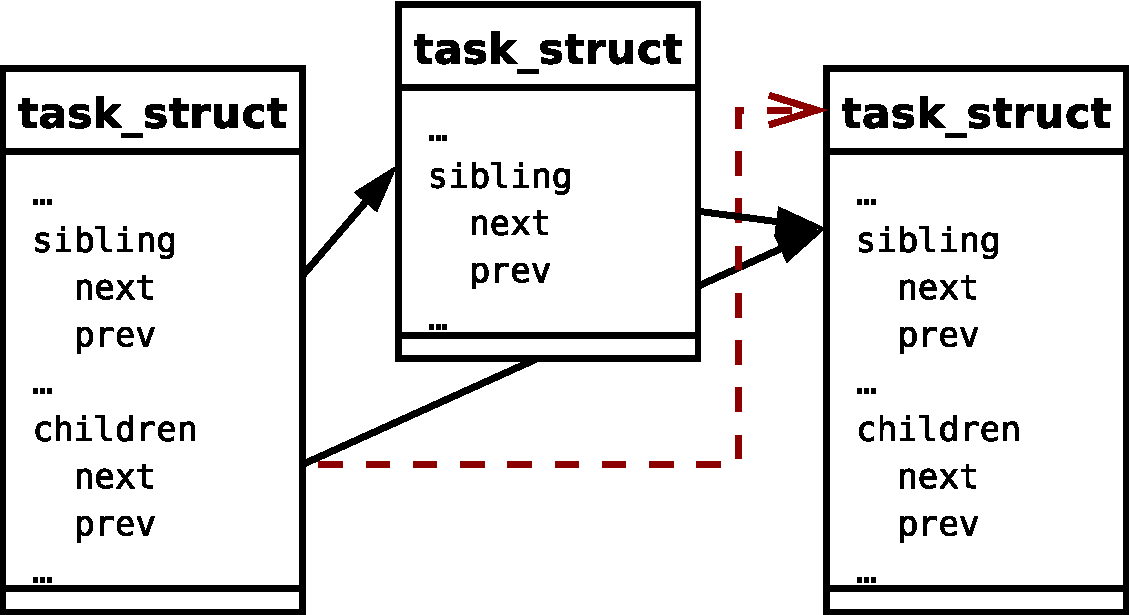
\includegraphics[width=8cm]{imgs/task_struct_illustration-crop.pdf}
    \end{center}
	
	\caption{Illustration of references used by linked lists in a \texttt{task\_struct}}
	\label{fig:task-struct-image}
\end{figure}
The example in listing \ref{lst:linkedliststypes} and figure \ref{fig:task-struct-image} can be used to illustrate the procedure:
A loop over all elements in a list is a frequent task.
\texttt{c} is the current element and its type \texttt{struct task\_struct} is the target object, i.e.~after the process, the tool should be able to do pointer magic such that \texttt{children.next} points to a \texttt{struct task\_struct}.
For now we do not know that \texttt{children.next} points to the \texttt{sibling} attribute of a \texttt{struct task\_struct}.
The usage of the macro however gives us the information: the last parameter is the name of the attribute inside the destination type.
The second attribute \texttt{\&p->children} gives us information for which member this association will be valid.
Again we use the debug symbols to find out that \texttt{p} is a \texttt{struct task\_struct} whose \texttt{children}’s attribute is then accessed.
\newline
Using this procedure, the mapping from \texttt{task\_struct.children} to \texttt{task\_struct.sibling} is established.
When accessing \texttt{children.next} we then know, that the pointer needs to be modified to subtract the offset of \texttt{sibling} within \texttt{task\_struct} to get a pointer to an actual \texttt{task\_struct}.

This approach yields considerable results: out of roughly 700 linked-lists 300 are auto-associated and the 
regular-expression based source-lookup tool could still be improved a lot to increase coverage. Nevertheless, 
there are a number of remaining structures for which the self-referencing heuristic mentioned earlier might 
not be valid and to which we do not gain access.

\subsection{Hashtables}
Even more troublesome than linked lists are hashtables, because the simple heuristics that have been helpful for linked-lists cannot be applied.
A hashtable is usually an array of \texttt{struct hlist\_head} elements which are entry elements (pointers) to a linked list of items in this bucket of the hashtable.
Each such item is represented by a \texttt{hlist\_node} structure which is a linked list similar to the \texttt{list\_head} structure. These nodes are also embedded into other data structures.
\begin{lstlisting}[frame=single,caption=Headed linked lists as used in the linux kernel,label=lst:hlists]
// first --> | next | -->  | next | -->  | next | 
//           | prev |  <-- | prev |  <-- | prev |
\end{lstlisting}
However there is no reference which structures belong to the \texttt{hlist\_node}s of a given hashtable array.
As it turns out though, the usage of the macro \texttt{void hlist\_add\_head(struct hlist\_node *n, struct hlist\_head *h)} establishes a connection between a \texttt{hlist\_head} instance and the corresponding \texttt{hlist\_node} structure.
While this macro and its use is not accessible from the debug symbols, it is quite grepable from the source.
We did not yet implement an automated approach, but feel confident that the same techniques we used to auto-associate linked lists can be used here to auto-associate the corresponding parent structures
(those that include \texttt{hlist\_head}, \texttt{hlist\_node}).
We can then use the generated mapping to implement an abstract Hashtable data type that takes these specialities into account.
Also a manual approach might succeed, as it seems there are less than 50 different hashtables in the kernel.

As long as the hashtable-handling has not been implemented, heuristic workarounds may be used, % in the meantime,
although these dirty approaches have significant drawbacks and should only be used to overcome the time until the hashtable-mappings are present.
There is an upper bound for structures including those hashtable nodes, which never exceed 2048 bytes.
Thus while the specific semantics of a memory region belonging to a \texttt{struct hlist\_node} are unknown,
it is known that up to 2048 bytes are being used to store information. As such, comparing memory can go ahead and compare the raw bytes,
trying to find out what changed.
Unfortunately all hashtable nodes also contain pointers, indicating that there is more information belonging to a node and that this information is not stored within the node itself.
Since the semantics of the memory region are unknown, we are likely to miss entry points to other memory structures when restricting hashtable node comparison to the very local memory only.

Hashtables in the kernel are usually used to store data, but most likely do not store very sensitive data or provide entry points to huge memory regions which would be missed if the references from the hashtable would not be followed.
As such it seems reasonable to skip hashtable handling in a first approach completely.

\subsection{Arrays and Pointers}
It is common convention to declare Strings as \texttt{char}-pointers (\texttt{char *}), however in the data model, a \texttt{char *} is a pointer to a \texttt{BasicType} instance \texttt{char} which is exactly one byte long.
While this knowledge is used to convert all \texttt{char}-pointers to a String meta-type, it is not clear what should be the behaviour for other types, as \texttt{int *} might also reference an integer field.
However, even if the integer field is correctly declare as \texttt{int field[]}, the length is still unknown,
leaving it for the program to guess or \emph{know}.
There seems no easy way to overcomes this problem, but to ignore all the data in the field unless one uses manual approaches:
Usually the array’s length is indirectly known: be it a static configuration or another member of a \texttt{struct}.
It is then no problem to override the array’s length by type-casting to an \texttt{Array} of a specified length.
There is also a \texttt{NullTerminatedArray} class which assumes a \texttt{NULL} entry to be the end delimiter,
which might be the case for many of those arrays with unknown length information.

	\section{Memory Access}
Having analysed the kernel symbols, we now know where data of which type is located in memory. 
Unfortunately the addresses found are virtual. The concept of virtual memory means that the physical 
locations within the built in memory chips are not accessed directly. Before accessing a virtual address 
location an address translation has to be done, which, in the case of a normal running system, 
is done automatically by the memory managing unit (MMU). 

In Linux 2.6 there are two main regions of virtual kernel space memory. One part from address 
\texttt{0x0000000000000000} to \texttt{PAGE\_OFFSET-1} (which is \texttt{0xffffffff80000000-1} 
\footnote{This numbers are valid for Kernel 2.6.27 and 2.6.28 with the default configuration 
on x86\_64 architecture.}), which can be accessed using the standard paging technique (\ref{paging}), 
the other part from \texttt{PAGE\_OFFSET} up to \texttt{0xffffffffffffffff}, is addressed using a 
linear address translation.

\subsection{Flat Kernel Memory}
\label{flat_kernel_memory}
The virtual memory area from \texttt{PAGE\_OFFSET} upwards is again divided in to two different regions. 
One from \texttt{PAGE\_OFFSET} upwards, and one from \texttt{\_\_START\_KERNEL\_map} 
\footnote{which is \texttt{0xffffffff80000000} in Linux 2.6.28 on x86\_64} upwards. 
In either case the starting address gets subtracted from the virtual address to acquire the 
physical address of the memory location inspected. All in all, we can say that regions for which 
the simple subtraction memory address translation is performed, are located in the beginning of physical memory.

\begin{lstlisting}[language=C,frame=single,caption=Accessing flat kernel memory and determine whether paging is required.,label=lst:flat_memory_access]
  if (virtual >= __START_KERNEL_map) {
  	return (virtual - __START_KERNEL_map);
  } else if(virtual >= PAGE_OFFSET) {
        return (virtual - PAGE_OFFSET);
  } else {
        // otherwise use the address lookup function
        return page_lookup(virtual);
  }
\end{lstlisting}

\subsection{Paged Kernel Memory}
\label{paging}
We have a completely different situation if we encounter paged virtual memory addresses.
Memory blocks, which are linear in virtual address space, may be distributed over several pages, which are not necessarily laid out linear in physical memory. Normally most of the kernel memory is linear accessible, because some devices that do direct memory access (DMA) require the memory region they are accessing to be linear not only in virtual, but also in physical address space. The only way to get a paged memory region in the kernel address space is to do a \texttt{vmalloc()}, which is mostly done when a bigger portion of memory is required, for example when inserting a kernel module.

When the x86\_64 machine encounters a virtual paged address, it looks up its physical page address in a page directory. 
Therefore the virtual address is divided into several parts, that index into the specific page tables (see figure \ref{page_table_structure}).

\begin{figure}[htb]
	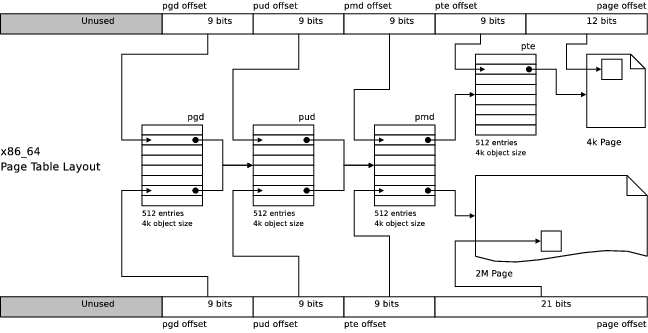
\includegraphics[width=0.95\textwidth]{imgs/x86_64_pagetable_structure.png}
	\caption{{\small Linux x86\_64 page table structure. Source: \url{http://linux-mm.org/PageTableStructure}}}
	\label{page_table_structure}
\end{figure}

As it can be seen in the figure there exist two types of pages: \texttt{4k} and \texttt{2M} pages. 
The only difference between them is their size and the indexing. For \texttt{2M} pages the last 21 bits 
of the virtual address are used to define an offset inside the page and the \texttt{pte} page directory is omitted. 
For \texttt{4k} pages the last 12 bits define a page offset and the 9 bits before that define an index 
into the 4-th level of page directory (\texttt{pte})

%Normaly this translation and lookup is done internally by a memory management unit (MMU) built into the processor. 
Since we want to access a physical memory image without having a MMU we have to emulate the accesses and 
lookups into the page directories. The entry point is the base address of the \texttt{pgd} directory. 
It is kept in the \texttt{\_\_ksymtab\_init\_level4\_pgt} kernel symbol. 
Then the virtual address is shifted successively and the lookups into the page directories are done. 

Additionally each page possesses several flags that have to be checked. One already mentioned, 
is the \texttt{PAGE\_2M} flag which identifies a \texttt{2M} page. Another important flag is the 
\texttt{PAGE\_PRESENT} flag, which is only set, if the page is allocated and available in physical memory. 
Otherwise the operating system would raise a page fault, to handle the situation accordingly. 
The third important flag would be the \texttt{PAGE\_SWAPPED} flag, which identifies that the page 
is not stored in main memory. Instead it is stored on some dedicated disk space (swap) and has to 
be loaded from there first. In our implementation swapped pages are not supported.

Every userspace program possesses its own virtual address space. Therefore separate page tables 
have to be held for each. Accessing this address is possible, if we know the process to which the address 
belongs and its pagetable location. Then a lookup can be done, just as in case of paged kernel addresses. 
In our work the focus is on analysis of kernel rootkits, therefore user space memory access is not implemented.

\section{Memory Image Comparison}
A central goal of this work is to watch memory of a virtual machine for changes and judge if malware (especially rootkits in this case) could be detected.
In order to accomplish this, two memory images (one taken before malware installation, one after) have to be compared. Usually one would compare the two physical memory dumps bytewise and try to guess if the changes happended in regions known to be security critical.
The drawback of this approach is, that one needs prior knowledge of the malware and manually create rules to detect specific malicious behaviour.
Unfortunately it is infeasible to define rules of yet unknown malware.
Therefore the opposite direction should be tried.

Instead of starting with binary differences of memory images, we start from the high level view of kernel symbols. 
For those we check whether the memory where they reside changed and if these changes reflect the behaviour of malware.

To perform a meaningful comparison two memory snapshots are opened at the same time, while our tool recursively inspects the situation: Each toplevel kernel symbol is added to a queue of symbols to compare.
The search is then conducted using a breadth first search algorithm.
Until now, the tool only reports if a specific symbol has changed.
In order to detect malware successfully, it may prove neccessary to compare the content of the changes, too.
Since the whole memory image is walked through by a python script the performance is still far from realtime. 

To implement realtime analysis for virtual machines while they are running, it could be possible that we again have to go the other way: 
Find the binary differences of the memory snapshots and abstract a high-level view of what changed without recursively checking every kernel variable.
Using our memory-coverage map, we are able to map a memory-location to a kernel variable and thus can get a list of changed variables when applying this technique to the locations found by the bin-diff tool.
While this map can be calculated in advance, this has some serious drawbacks that would need to be addressed beforehand.
If bare variables change, this is no problem, but for example in the case of pointers, 
the location of data pointed to could have changed, and therefore the value of the pointer.
This would invalidate all variables in the map to which the pointer is a parent node (in the chain from a global symbol to the variable).
One might then think of updating the mapping in iterative ways, however such algorithms remain yet to be implemented.


	\section{Rootkit Analysis Findings}
\label{rootkit_analysis}
% several rootkits analyzed: module_hide (change module linked list), taskigt (create proc files)
%		still to port: change system call table (difficult in kernel 2.6)
% analyze the changed toplevel symbol names
% analyze all symbol names
For each analyzed rootkit a snapshot has been taken before installation and after and the changed kernel symbols were listed.
We used this information to first of all check if
malicious behaviour of each different type of rootkit is reflected among all the changed symbols.
The following sections present our findings.

\subsection{Rootkit Types}
For a rootkit it is not only important to implement some specific services needed by the attacker, but 
also to make those capabilities accessible. At the same time the malicious module wants to hide itself 
and all its activities from the system administrator. To accomplish this, several hooking mechanisms 
into the kernel have to be established. Among the rootkits, that are public available, there are basically 
three different mechanisms of hooking into the kernel. One is to generate special files in the 
Virtual File System (VFS) like \texttt{proc}, another one is to modify kernel structures directly and 
the third and most commonly used one is to replace specific system calls in the system call table (\texttt{sys\_call\_table}).	

\subsubsection{System Call Replacement}
\label{system_call_replacement}
When using an operating system, 
the user must be able to perform system calls in order to invoke special kernel functionalities (for example listing 
and opening files). For this purpose the linux kernel manages a big array with function pointers to the system call 
functions implementing each functionality. 

If a programm invokes a system call (interrupt \texttt{0x80} on x86 architectures), the interrupt dispatcher looks up 
the desired function in the \texttt{sys\_call\_table} and calls it. Until kernel version 2.6 the \texttt{sys\_call\_table} 
was among the exported symbols that could be used by loadable kernel modules. Therefore it was easy to replace the 
function address by an address of a function that intercepts the system call to, for example, filter out specific 
files from directory listings in order to hide the rootkit itself. 

Since Kernel 2.6 the syscall table symbol was no longer exported and the rootkit authors had to invent new ways 
of finding the table location:

\begin{enumerate}
	\item {\b Kernel Memory Search}: With this method the memory area between \texttt{init\_mm.end\_code} and 
		\texttt{init\_mm.end\_data} (which is basically the \texttt{\_text} segment of the kernel image), 
		is searched and the contents are compared to the addresses of known system call functions. 
		Since we know where the specific system call function, we searched for, is located in the system call table, 
		we can calculate the start address.

	\item {\b Interrupt Handler Search}: On the x86 architecture there exists the \texttt{sidt} instruction. 
		This instruction gives us the address of the interrupt vector table. We know that for calling a system call 
		the \texttt{0x80} interrupt is raised and the appropriate interrupt handler calls the right system call 
		function for us. Since the handler has to know there the table with all the system calls is located, 
		we can search in the memory section, where the handler resides for the actual function call and extract 
		the start address of the \texttt{sys\_call\_table} from there.

	\item {\b Compile Time}: A third technique is to use the address known from \texttt{System.map} at compile time. 
		In this case we have to be able to compile our rootkit on the machine where we want it later to be run. 
		We also have to have access to the \texttt{System.map} to lookup addresses. Eventually a module
		could also find out the syscall table address at load by looking it up in \texttt{/proc/kallsyms}.
		In our tests this is the method we used.
\end{enumerate}

On newer 2.6 kernels it is not sufficient to find the system call table. Several protection mechanisms have been employed: 
The pages where the table resides is flagged as read only. 
Trying to change that with the \texttt{set\_memory\_rw} function will fail since this function also has some 
protection built in. But a kernel hacker is still able to modify this part 
of memory: Since we cannot use the kernel functionality to change access rights of memory sections, we have to implement 
them ourselves. Walking the page tables and changing flags could be implemented in the loadable kernel module itself.

Detection of such modifications are possible with our tool. It detects all changed function addresses in the table. 
One rootkit we inspected did even go further than just replacing function pointers: It did not replace the system call 
table itself, but it first copied it and modified the copy. Then the interrupt handler for system calls was modified 
to use the new system call table. Such a modification is not yet detected by our tool, since we do not yet take
registers into account as global symbols. Thus the tool still uses the address 
of the old table, which stays unmodified. If we are inspecting a virtual machine the machine registers have to be
considered as well.

\subsubsection{VFS Manipulation}
The virtual file system is an additional layer on top of all the file systems implemented in Linux. 
It enables the user to uniformly access his files independently of the underlying file system. One special 
file system present in Linux, is the \texttt{proc} filesystem. It was implemented to give access to 
kernel and loadable module parameter configuration or to access debug information present in the kernel. 

The file entries in the proc file system are different from ordinary files. On access of such an entry, 
there is no read from a block device. Instead a function call to a specific function associated with that 
file node is called. Within this function the neccessary data can be generated and copied back to the user. 
Analog happens upon write access to the file. The data written by the user can be parsed and configuration 
parameters can be set accordingly.

One rootkit we analyzed used VFS manipulation to give root privileges to certain processes. To accomplish 
that a new file is created in the \texttt{/proc} directory. If a process accesses this file, the kernel function 
handling the read or write operation has access to a \texttt{task\_struct} structure of exactly that process. 
Therefore it is easy to modifiy the \texttt{uid, gid,...} members of that structure, which control the privileges.

Detection of such a modification can be done using our toolkit. The difficulty in this case lies in the 
classification of the changes. In our experiments we observed numerous proc filesystem modification during normal 
operation of the running machine. Just creating an entry in /proc is not neccessarily malicious. Changing the 
UID of a process can be, but can also happen during normal runtime (take \texttt{sudo} for example). 
Therefore unauthorised modification is very difficult to spot. One can try 
to match malicious behaviour by inspecting the filenames of the newly created files, but this name can easily 
be changed to something unsuspicious by the attacker.

\subsubsection{Direct Kernel Object Modification}
Most of the rootkits did hide themselves by system call interception 
and filtering of the results as described in section \ref{system_call_replacement}. 
Another technique is to modifiy the kernel structures directly. Of course malicious 
attacks other than just hiding can be achieved with direct kernel object modification.

\begin{figure}[htb]
	\begin{center}
	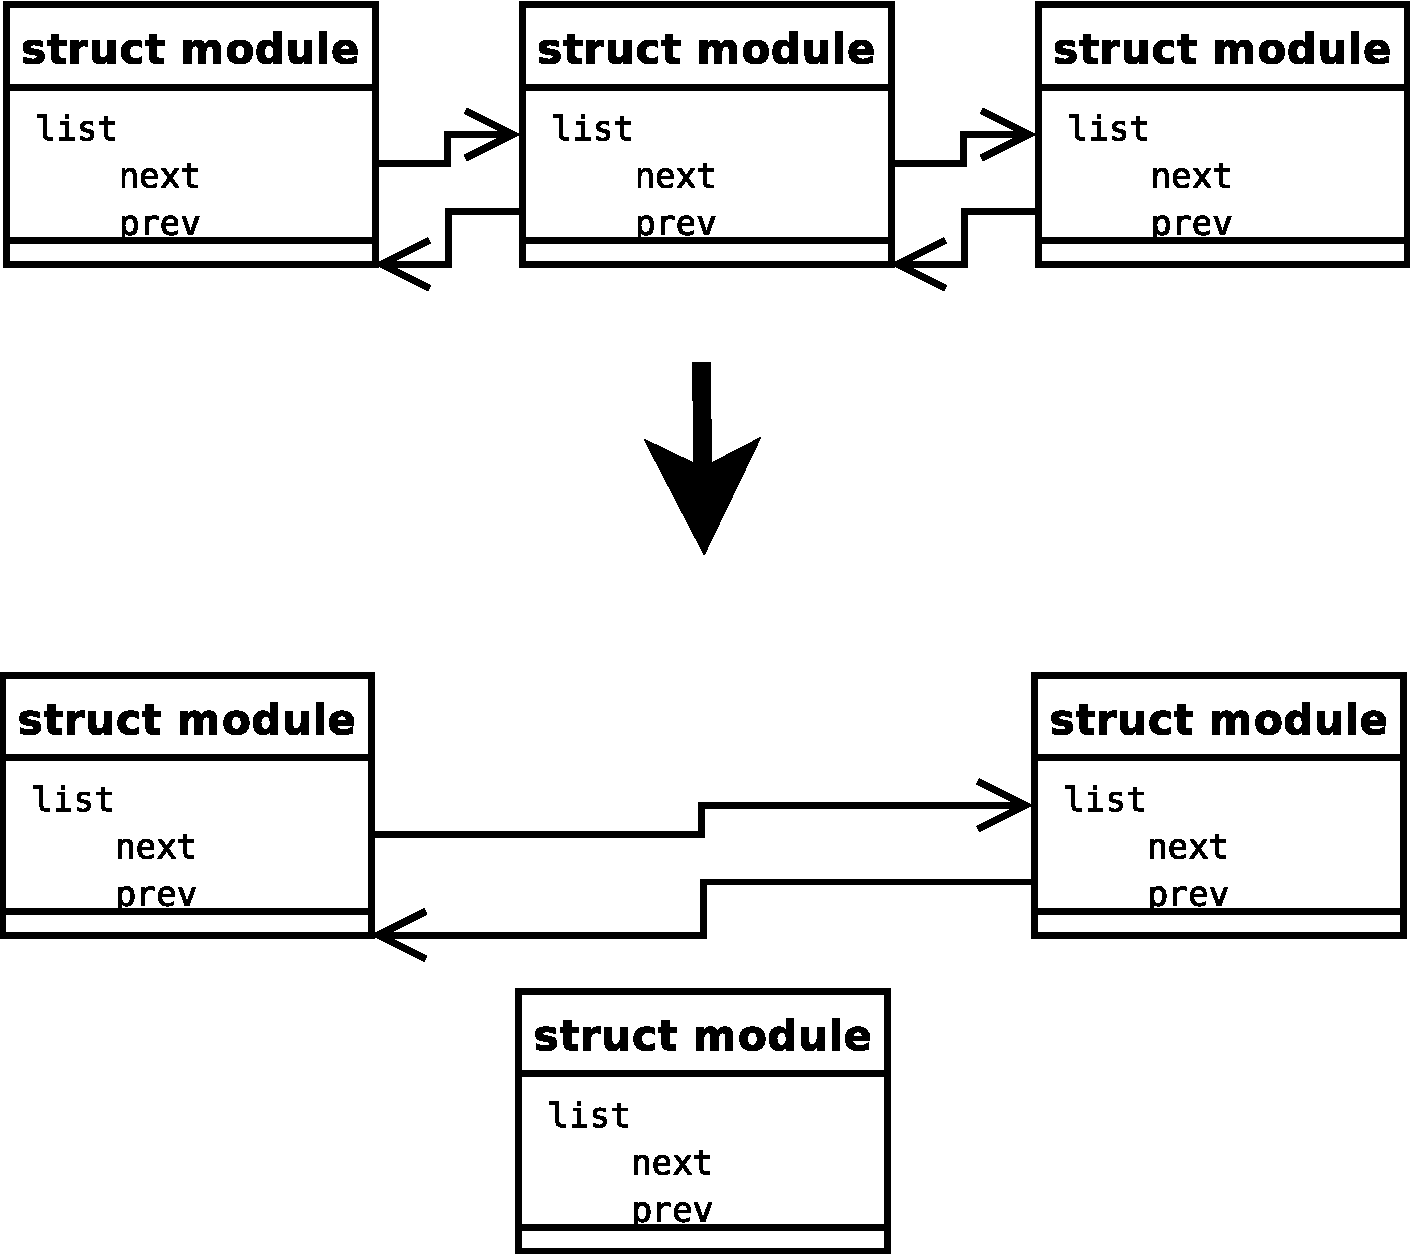
\includegraphics[width=0.45\textwidth]{imgs/module_list_modification.pdf}
	\caption{Skipping a module in the internal kernel module list.}
	\end{center}
	\label{skip_module}
\end{figure}

For keeping track of all the loaded modules, the kernel manages a double linked list. The kernel system 
calls that deal with modules (e.g. \texttt{insmod}), make use of this list. 
If the user requests to unload a specific module from the kernel, first the module list is searched 
for one with the specified name, then this reference is taken, unloaded and removed from the list.

If the attacker now removes a specific module (see figure \ref{skip_module}) from the internal list, by just 
updating the pointers (see figure \ref{skip_module}) and thereby skipping one entry in the double linked list, 
the kernel itself has no more access to this. Removing and other access to this module is no longer possible. 
Also the module does not show up on \texttt{lsmod}, which was the intention of the modification. 
Another fact is that all the hooks and callbacks, the malicious module may have placed into the kernel, still exist 
and the module itself still resides in memory. Therefore the normal operation of the rootkit is available, while 
unloading and listing is not possible.

Detecting such modifications is possible with our toolkit. We are able to monitor all changes of kernel structures. 
For double linked lists, the list has to be traversed and all the entries analyzed (though the current version 
still has some problems fully dealing with linked lists). To be able to successfully detect an attack on kernel 
structures, we have to further analyze the changes. It could be possible that the module list has changed, 
because we loaded a kernel module by hand. These kind of changes have to be filtered out. 

Another difficulty in detecting such modifications are big timesteps between two analysis. If we take one 
snapshot before the malicious rootkit is loaded and one far after the module is completely loaded and 
already hidden, then we will see no changes in the module list. The module already vanished and cleaned 
itself up, leaving no direct traces for us to analyze. We still can search the memory for placed hooks 
into the kernel, which have to be there in order for the rootkit to function correctly.

\subsection{Analysis Conclusions}
Most of the modifications done by the studied rootkits can be identified with our method. 
The big challenge is to distinguish between malicious and normal changes of kernel structures. 
In the case of proc file system modifications we could find 
more modifications by just running a xterminal with some commands then by inserting the tested rootkit.

When supervising a virtual machine, it is also neccessary not only to monitor the memory, but also the special registers 
of the virtual cpu. Then even modifications of the interrupt handlers and with that copies of the system call table can 
be detected.


\begin{appendix}
  \section{Usage Instructions}
\begin{description}
    \item[Compilation]
	Adjust the path to the kernel source in your \texttt{Makefile}.
	Then, use the \texttt{make} command to compile the C modules required by the python package.
    \item[Kernel Preparation]
        A kernel image with debug symbols must be compiled or obtained.
        Afterwards \texttt{objdump} can be used to extract the debug-symbols in a textual format readable by the tool.
        Pay attention to use a recent version of objdump, as older ones might fail to read debug-symbols.
        Next, the type\_parser script is used to create the initial cleaned-up data model.
        As noted earlier this last step may take some time.
        It will save its results in the data.dumpc file, which is later used to quick load the data model.
        \begin{lstlisting}[frame=single,caption=Initialisation Workflow,label=lst:workflow]
 # objdump -g vmlinux > vmlinux.dbgdump
 # python type_parser.py init vmlinux.dbgdump
        \end{lstlisting}
    \item[Additional Information Acquirement]
	Certain information is not available in the kernel’s debug symbols.
	Linked lists have been implemented and require an additional setup step to work correctly:
        \begin{lstlisting}[frame=single,caption=Linked List Initialisation Workflow,label=lst:workflow]
 # python type_relater.py /path/to/compiled/kernel/source meta_info.dump > /dev/null
        \end{lstlisting}
    \item[Memory Unlocking]
        In order to access the \texttt{/dev/mem} device without any restrictions, the supplied memunlocker kernel module needs to 		be loaded: \begin{lstlisting}[frame=single,caption=Unblocking /dev/mem,label=lst:unlocking]
 # sudo insmod memunlocker/memunlocker.ko
         \end{lstlisting}
    \item[Using the Shell]
	Interactive kernel symbol exploration can be done via the python shell. First of all the precalculated debug symbol data 		has to be loaded. Then a memory image (can be the \texttt{/dev/mem} device or a physical memory dump of a virtual machine) 		is mapped using the memory.c python plugin.
	\begin{lstlisting}[frame=single,caption=Starting up interactive shell,label=lst:shellstartup]
 # python
 >>> from tools import *
 >>> types, names, addresses = init(memory_image, parents=True, linked_lists=True)
 >>> it = kernel_name('init_task')
 >>> init = it.children.next
 >>> init
 <Memory <c_types.Struct instance 'task_struct'> @0xffff88001ccc8000>
 >>> init.pid
 <Memory <c_types.Member instance 'pid'> @0xffff88001ccc8268>
 >>> print init.pid
 1
 >>> 
	\end{lstlisting}	

    \item[Symbol Comparision]
	In order to be able to compare a symbol at different time snapshots, a second memory dump has to be mapped. 
	Then the location of the level 4 page table directory has to be published to the memory python module.
	\begin{lstlisting}[frame=single,caption=Mapping a second memory image,label=lst:map]
 >>> memory.map(second_image, filesize, mapsize (usual same as filesize), 1)

 >>> pgt = kernel_name('__ksymtab_init_level4_pgt')
 >>> memory.set_init_level4_pgt(int(pgt.value.get_value()))
	\end{lstlisting}
	If everything is set up symbols can be compared by first getting a reference with \texttt{ref = kernel\_name('symbol')} and 		then using the \texttt{memory\_manager's} \texttt{.memcmp()} functionality: \texttt{ref.memcmp()}.
	For a complete example see \texttt{diff.py}.
    \item[Report generation]
	Several components are capable of generating (more or less) detailed reports on actions and failures.
	This information will be of great use for improving the tool and debugging errors it might have made.
        \begin{lstlisting}[frame=single,caption=Generating Reports,label=lst:workflow]
 # python troubles.py           > reports/trouble-areas.xml
 # python type_relater.py /path/to/kernel/source meta_info.dump \
                                > reports/linked-lists-parsing.xml
 # python tools/linked_lists.py > reports/linked-lists-autoassociate.xml
        \end{lstlisting}
\end{description}

\end{appendix}

%%%%%%%%%%%%%%%%%%%%
%\newpage
%\bibliographystyle{natdin}
%\bibliographystyle{natbib}%unsrtain,alpha
%\bibliography{literature}
\end{document}
